% SPDX-FileCopyrightText: Copyright © DuMux-Lecture contributors, see AUTHORS.md in root folder
% SPDX-License-Identifier: CC-BY-4.0

\documentclass[12pt,twoside]{article}

% some packages used
\usepackage{amsmath}
\usepackage{amsfonts}
\usepackage{epsfig}
%\usepackage{psfig}
\usepackage{makeidx}
\usepackage{chicago}		% for bibliography style needed
\usepackage{fancyvrb}		% for Verbatim enviroment
\usepackage[english]{babel}	% for name of figures, tables
\usepackage{rotating}
\usepackage{longtable}
% some needful macros

%\include{macros}

% some settings for the pageformat
\textheight 21cm
\textwidth 16cm
\footskip 8mm
\oddsidemargin 0mm
\evensidemargin 0mm

\parindent 0pt

%%%%%%%%%%%%%%%%%%%%%%%%%%%%%%%%%%%%%%%%%%%%%%%%%%%%%%%%%%%%
\begin{document}
\sffamily
\pagenumbering{roman}

%\maketitle

%\cleardoublepage

\setcounter{tocdepth}{4}	% prints toc down to 4 levels
%\tableofcontents
%\listoffigures
%\listoftables

%\cleardoublepage

\pagenumbering{arabic}
\pagestyle{plain}
\setcounter{secnumdepth}{4}	% allows numbers for sub-sub-section

% SPDX-FileCopyrightText: Copyright © DuMux-Lecture contributors, see AUTHORS.md in root folder
% SPDX-License-Identifier: CC-BY-4.0

\section{The Heatpipe Effect}
\subsection{System Description}


The Heatpipe Effect is described by a nonisothermal water-gas system 
in a porous medium, in which the heat transfer processes
convection, conduction, and diffusion as well as capillary forces play
an essential role. 
Udell and Fitch (1985) \cite{Udell:1985} provide a semi-analytical solution for this system, 
which is practical for comparing with numerical results (e.g., see Emmert, 1997
\cite{emmertpromo}).
\begin{figure}[h]
    \centerline{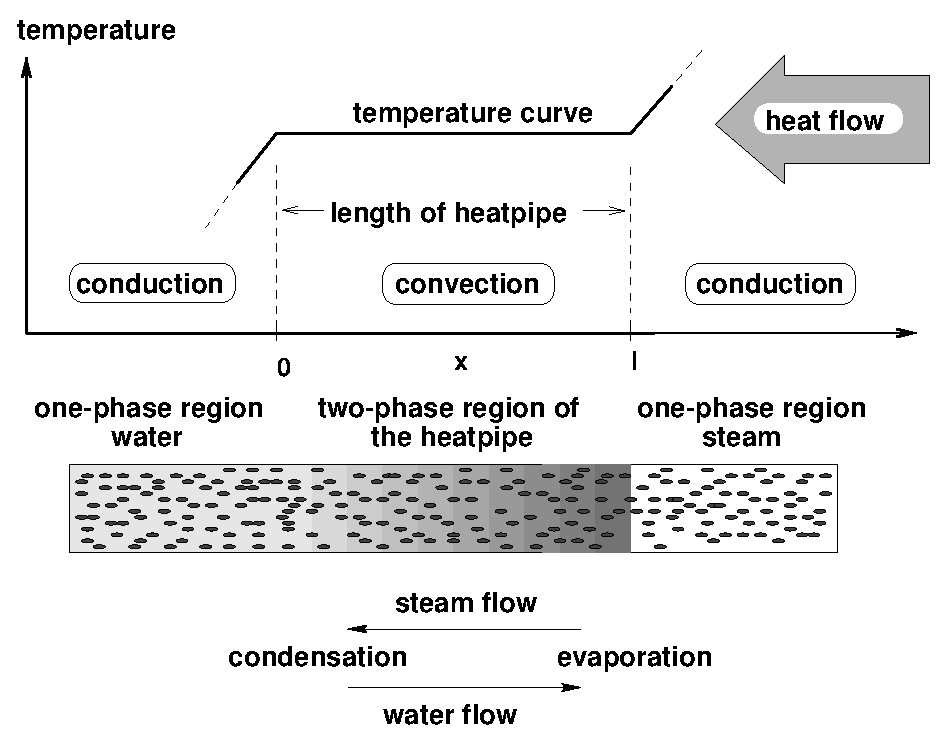
\epsfig{file=eps/121phasc_sw.eps,width=0.6\textwidth}}
    \caption{The heatpipe effect: schematic description}
    \protect\label{121phasc}
\end{figure}
A constant heat flux ($q = 100$W) into the column and a zero-flux condition 
(Neumann condition) for all mass components are given at the 
right-hand boundary of a horizontal column (Fig. \ref{121phasc})
with an initially constant water saturation of 0.5.
At the left-hand boundary, we have constant values (Dirichlet 
conditions) for the gas-phase pressure ($p_g = 101330$Pa), the 
effective water saturation
($S_{we} = 1.0$), and the air mole fraction in the gas phase
($x_g^a = 0.71$). Thus, the temperature,  
given as a function of $S_{we}$, $p_g$ and $x_g^a$ is also stated at $T = 68.6^\circ$C.:
\begin{equation}
T = \frac{ T_0 \left( 1 + \frac{p_c - x_g^a p_g}{h_v^w \varrho_w}
\right)}{1-T_0\frac{R}{h_v^w M^w} \, \mbox{ln} \left( \frac{p_g
(1 - x_g^a)}{p_0} \right)}
\end{equation}
Due to the heat flux, the system is heated until boiling temperature
is reached and steam is produced at the right-hand boundary. This causes
a pressure gradient in the gas phase and the steam flows away from
the heat source. After reaching cooler regions of the column, the steam
condenses and sets free its latent heat of vaporization. After a while,
a non-uniform saturation profile is obtained with a gradient from the 
cooler to the hot end of the heatpipe. According to the capillary 
pressure--saturation relationship a gradient of the
capillary pressure into the same direction is produced. Hence, the pressure gradients of the
phases have opposite directions and a circulation flow is created.
After a stationary system state has been reached, three regions can be 
distinguished, each of them associated with a dominant heat-transport 
process (Fig. \ref{121phasc}). 

Udell and Fitch (1985) \cite{Udell:1985} derive four
coupled first-order differential equations for pressure, saturation,
temperature and gas-phase mole fraction. These equations are solved
by numerical integration by means of a fourth-order Runge--Kutta method. 
The numerical simulation of the heatpipe system was carried out
with the BOX discretization method. Note that the choice of
BOX or CVFE makes no difference in the present one-dimensional
case. For the simulations, the upwind-technique for weighting the
mobilities and mole fractions at the interface between two boxes
has been switched off since upwinding cannot be considered in the
analytical solution.
The following model parameters were used for the simulation run:
\begin{tabbing}
\hspace{0.5cm} \=
Permeability \hspace{4.5cm} \= : $K=10^{-12}$ m$^2$ \\
\> Porosity \> : $\Phi=0.4$\\
\> Residual water saturation          \> : $ S_{wr}=0.15$\\
\> Heat conductivity of the \\
\> fully saturated porous medium \> : $\lambda_{pm}^{S_w=1}=1.13$
W/(m K) \\
\> Heat conductivity of the \\
\> dry porous medium                \> : $\lambda_{pm}^{S_w=0}=0.582$
W/(m K) \\
\> Soil grain density            \> : $\varrho_s =2600$ kg/m$^3$\\
\> Spec. heat capacity of the soil grains  \> : $c_s =700$ J/(kg K) \\
\> Density of water \> : $\varrho_w = 958.4$ kg/m$^3$ \\
\> Dynamic viscosity of water \> : $\mu_w = 2.938 \cdot 10^{-4}$ Pa s\\
\> Dynamic viscosity of air \> : $\mu_g^a = 2.08 \cdot 10^{-5}$ Pa s\\
\> Dynamic viscosity of steam \> : $\mu_g^w = 1.20 \cdot 10^{-5}$ Pa s
\end{tabbing}
A function according to Fatt and Klikoff (1959) \cite{Fatt:1959} is 
chosen for the relative permeability--saturation relationship:
\begin{eqnarray}
k_{rg} &=& (1 - S_e)^3 \quad \mbox{for steam (gas phase)} \nonumber \\
k_{rw} &=& S_e^3 \quad \mbox{for water} \, 
\end{eqnarray}
with the effective water-phase saturation
\begin{equation}
S_e = \frac{S_w - S_{wr}}{1-S_{wr}}\; .
\end{equation}
For the capillary pressure--saturation relationship, the following
function of Leverett (1941) \cite{lev1} is used:
\begin{equation}
\label{eqleve}
p_c = p_0 \cdot \gamma \cdot 1.417(1-S_e) - 2.120(1-S_e)^2 + 
1.263(1-S_e)^3 \, .
\end{equation}
The surface tension $\gamma$ at $T = 100.5$$^\circ$C is 0.05878 
Nm$^{-1}$
and $p_0 = \sqrt{\phi/K}$ applies for the scaling pressure. A constant
value of 0.5 is assigned to the tortuosity $\tau$ and the binary 
diffusion constant $D_g^{aw}$ takes the value $2.6 \cdot 10^{-6}$ 
m$^2$/s. \\
The dimension of the model domain in x--direction is chosen at 2.4 m.
However, this is not important for the length of the heatpipe after the
stationary state has been reached as long as the domain is 
sufficicently large
for the heatpipe to be built. We used a discretization length of
$\Delta x = 0.04$ m. The initial conditions were chosen to
$p_g = 101330$ Pa, $S_w = 0.5$ und $T = 70$$^\circ$C.
The results of the numerical simulation with the semi-analytical 
solution are compared in Figs. 2, 3, and 
4. In all cases, the curves match very well. 
A length of $\approx$ 2.0m is obtained consistently for the heatpipe.
Due to the complex interaction
of different physical processes and the excellent agreement between the
simulation and the semi-analytical solution, we state that the 
verification of the numerical model for an air--water system was 
successful.
With the given initial conditions, the model could reproduce
the heating at the right-hand boundary from 70$^\circ$C up to
boiling temperature. Also, the gradual extension of the heatpipe
region until the stationary system state was reached was modeled 
correctly.  The disappearance of the water phase associated with a 
change of the phase state and a substitution of the primary variables 
was carried out well. Fig. 4 shows clearly that the pressure 
gradients of both phases have different signs.

\begin{figure}[h]
    \centerline{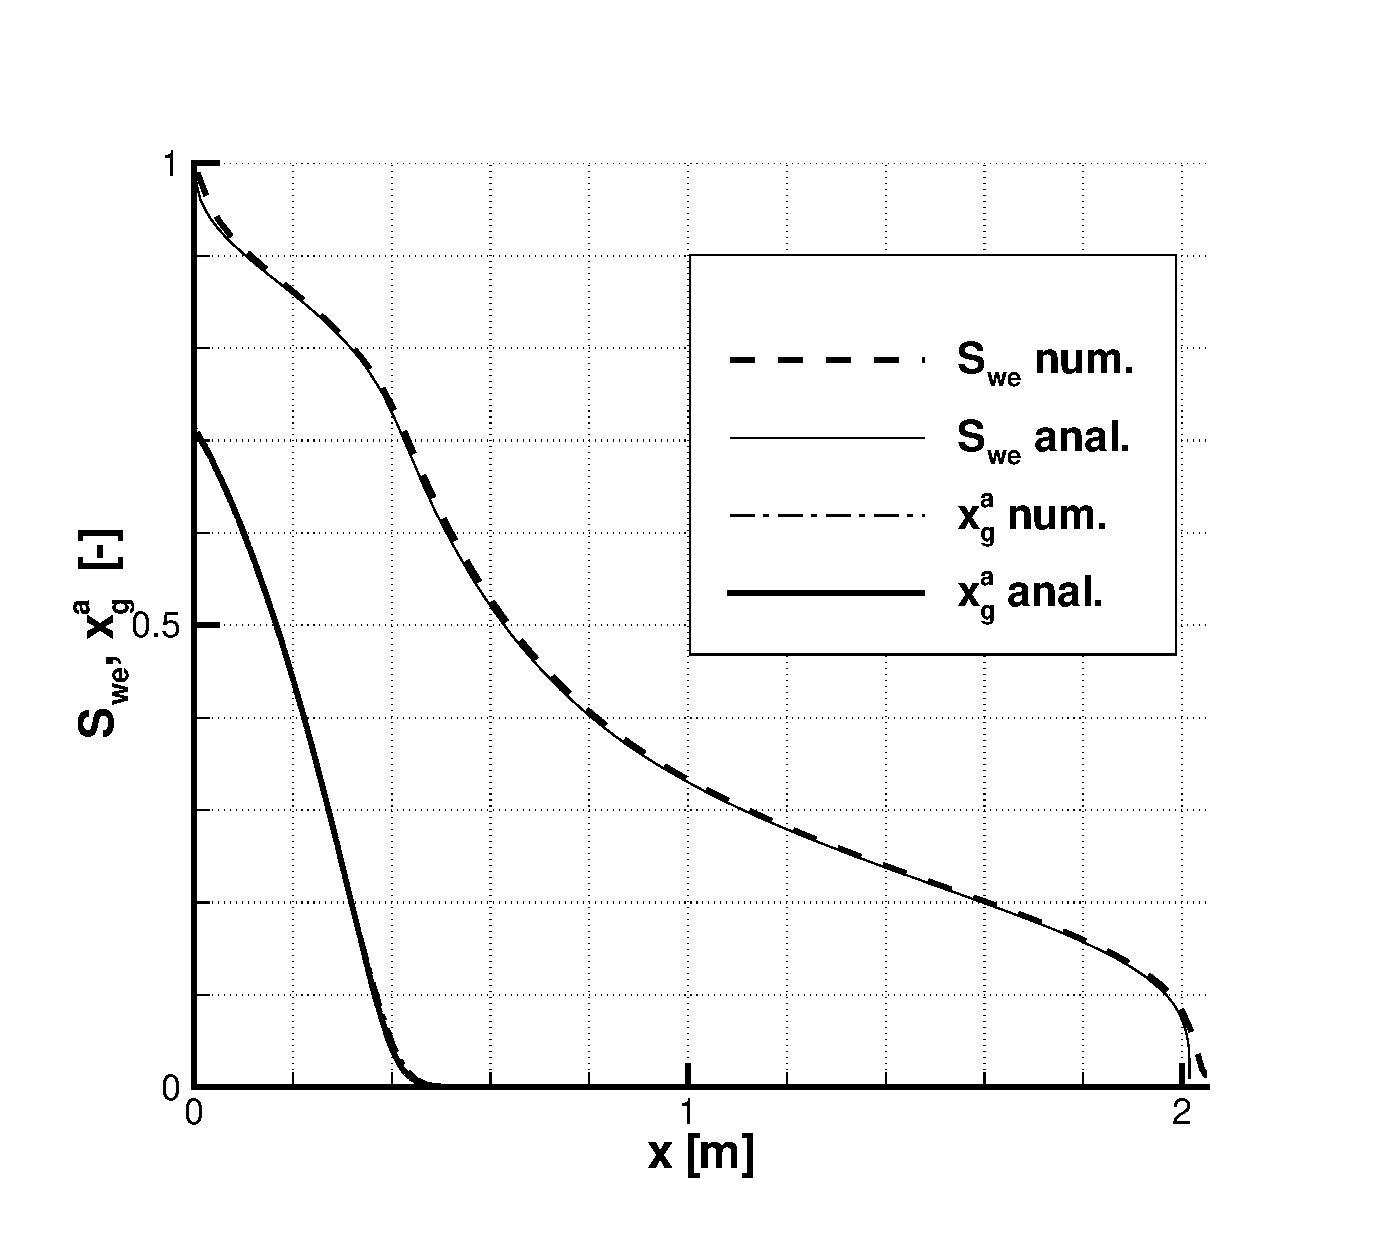
\epsfig{file=eps/swexag_sw.eps,width=0.70\textwidth}}
    \caption{Semi-analytical and numerical curve of $S_{we}$ and $x_g^a$}
\end{figure}

\begin{figure}[h]
    \centerline{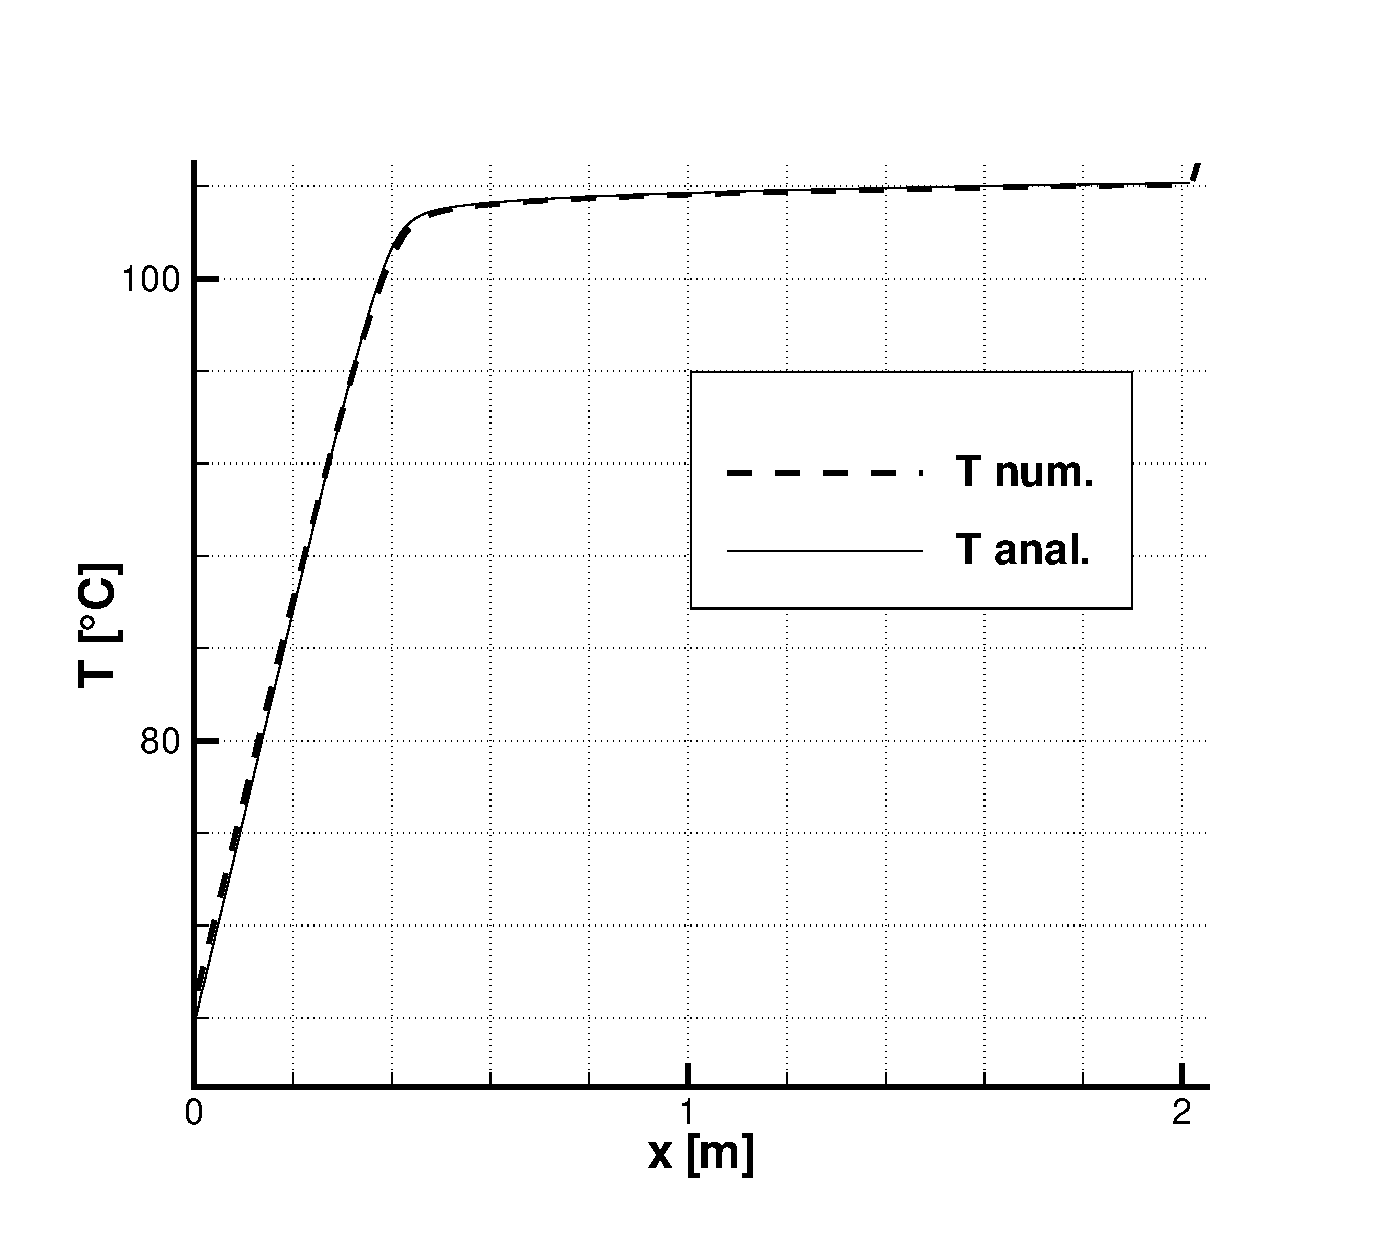
\epsfig{file=eps/temp_sw.eps,width=0.70\textwidth}}
    \caption{Semi-analytical and numerical curve of $T$}
\end{figure}

\begin{figure}[h]
    \centerline{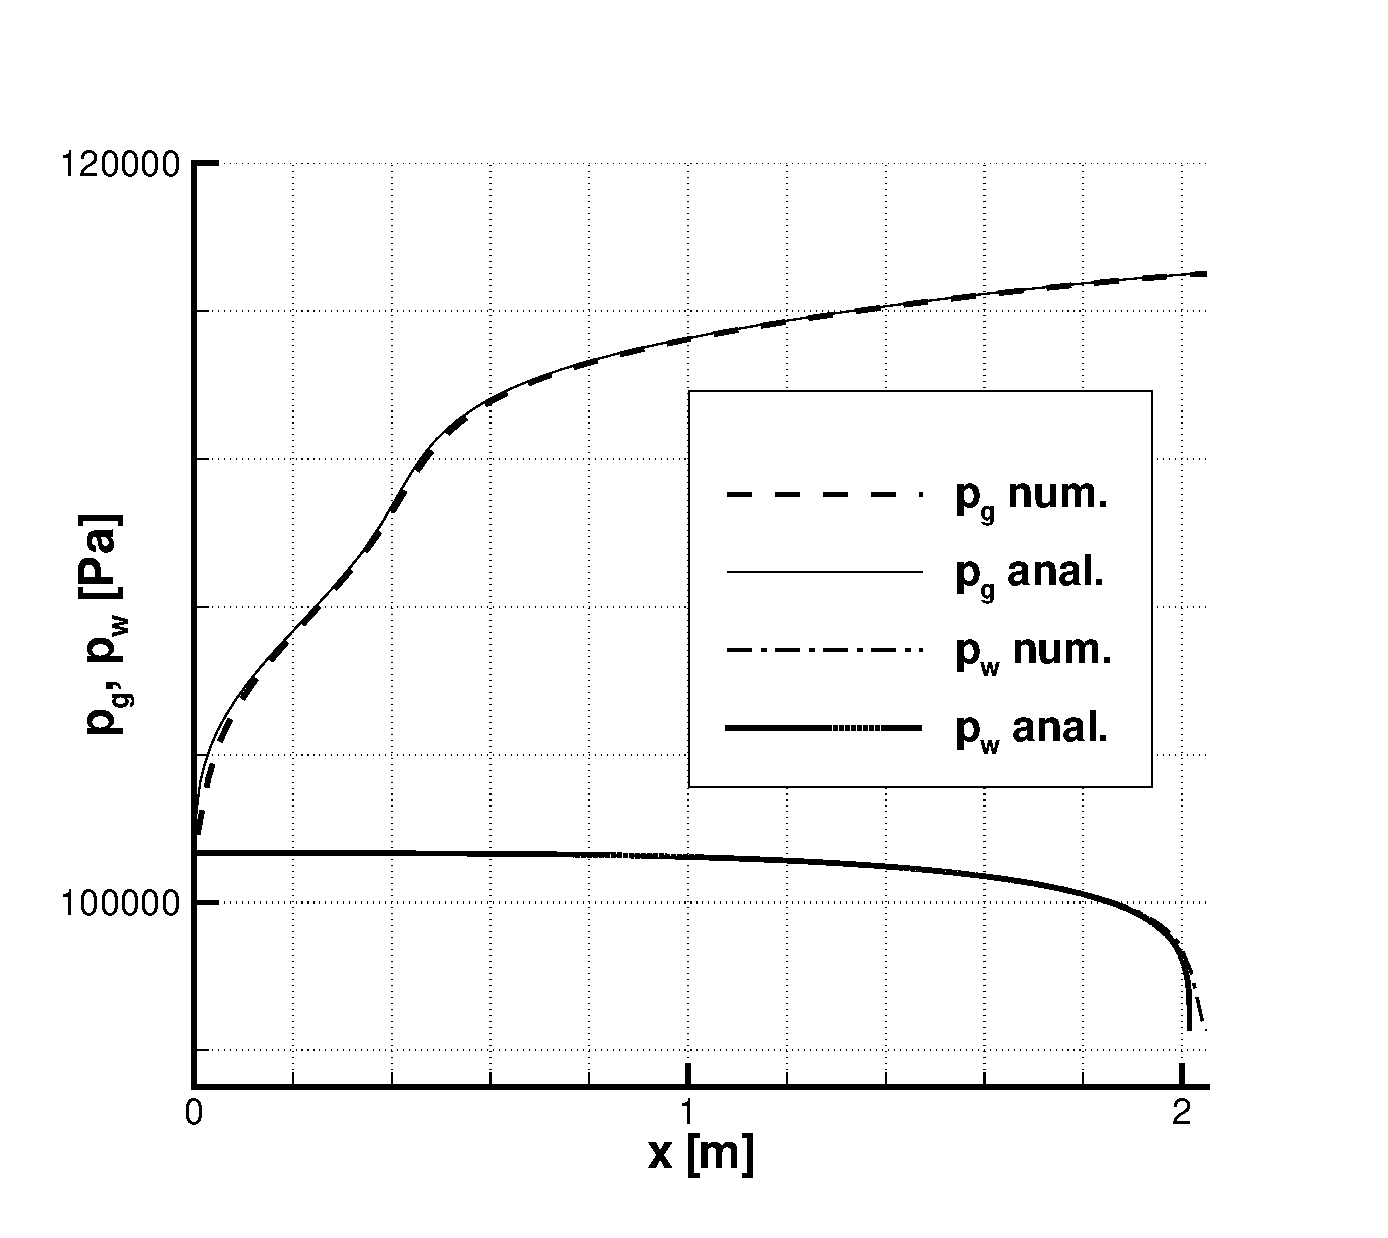
\epsfig{file=eps/pgpw_sw.eps,width=0.70\textwidth}}
    \caption{Semi-analytical and numerical curve of $p_g$ and $p_w$}
\end{figure}

\clearpage

\subsection{Paraview}
It is recommended to you use a Plot-Over-Line to display a cross-sectional view
on the parameters saturation, temperature, pressures, etc.

\subsection{Exercises and questions}

Compile and run the model by modifying one by one a number of parameters.
Usually, it is sufficient to use the parameters in the input file.

Keep attention to the length of the heatpipe. Dependent on the choice of the
parameters, it can be necessary to increase the length of the model domain if
you want to see the full heatpipe.

\begin{enumerate}
\item Which influence has the capillary pressure on the extension of the heatpipe?
\item Which influence has the heat source on the extension of the heatpipe?
\item What are the effects of a higher/lower heat conductivity of the porous medium?
\item How does the permeability of the porous medium influence the process? 
\item What happens when you replace the full upwinding by averaging in your
discretization scheme? To do 
this you have to add
\begin{tabbing}
\hspace{0.5cm} \=
\texttt{[Implicit]} \\
\> \texttt{UpwindWeight = 0.5}
\end{tabbing}
to your input file.
Compare the result with the analytical solution and with the solution you get with 
upwinding.
\item  Refine the mesh and run the program again with upwinding. To refine the mesh 
you have to increase the number of cells in your heatpipe.dgf file.\\
Are there any changes? Explain.
\end{enumerate}


\bibliography{heatpipe}
\bibliographystyle{plain}

%\cleardoublepage
\printindex

\end{document}
